\documentclass[../Head/report.tex]{subfiles}
\begin{document}
\section{Discussion}
\label{sec:discussion}

\subsubsection*{Initial pose estimation using the GPS to vision ArUco board}
From the results in Section \ref{sec:GPS2Vision_pose_estimation} a circular region of poses where the ArUco pose estimation error is quite low was found to be within a maximum distance of approximately 5 meters away from GPS2Vision board. The errors can be seen to be high when the UAV is approximately 5-8 meters away, or more, from the GPS2Vision board which goes for both position and angle. From these observations, a safe area for the transition between using GPS to vision as navigation would be within a radius of approximately five meters away from the GPS2Vision board which can be seen in Figure \ref{fig:GPS2Vision_pose_estimation_test1_error_pos} and \ref{fig:GPS2Vision_pose_estimation_test1_error_ori}. 

A possible reason why especially the z position deviates a lot when moving away from the board is that the z component in the coordinate system moves with an angle in roll which triggers the altitude of the UAV to go from positive to negative and hence increases the error in z more than x and y which are less sensitive according to the analysis. It is also quite interesting to see that the position in z is more sensitive when moving away from the board when being straight in front of it. This can be seen in Figure \ref{fig:GPS2Vision_pose_estimation_test1_error_z}. By being further away from the board does not yield the same kind of sensitivity for the position in x and y, but they are more sensitive when facing the board by having an angle in yaw as seen in Figure \ref{fig:GPS2Vision_pose_estimation_test1_error_x} and \ref{fig:GPS2Vision_pose_estimation_test1_error_y}.   

Based on the results, the maximum distance away from the GPS2Vision board when executing the GPS to vision transition should not exceed five meters with the current configuration of the ArUco marker board and resolution of the camera which was set to $640 \times 480$. However, it is possible to reduce the errors by having a better resolution because the detection of markers would be more precise due to the fact the more pixels would yield a better separation of the borders of the markers which in turn produces better pose estimates. This could yield a better performance of the system, but may also stress the Raspberry Pi in regard to calculations performed. A way to accommodate for that is to use a stronger companion computer e.g Jetson nano, which comes with the expense of a higher price.

\subsubsection*{Analyzing rolling average for fluctuations in the pose estimation}
As it can be seen in Figure \ref{fig:rolling_average_pos_test1} and \ref{fig:rolling_average_angle_test1} in Section \ref{sec:rolling_average_aruco_pose_estimation}, the fluctuations in the estimates are only of minor concern when the UAV is of a maximum distance of 5 meters from the GPS2Vision board. However, when the UAV changes to a position being more than five meters away from the GPS2Vision board, the estimations in position fluctuates a lot as seen in Figure \ref{fig:rolling_average_pos_test2}. This could be fatal to make a transition in this scenario and lead to an unstable system. The estimation of the orientation of the UAV is affected less as seen in Figure \ref{fig:rolling_average_angle_test2}. Hence, the outcome of the rolling average has been used alongside the maximum distance to the GPS2Vision board for stability analysis before initiating the GPS to vision transition. 

One may argue that being close enough to the ArUco marker board should be a valid criteria for this transition, but for safety precautions this extra criteria has been considered in the implementation. Nonetheless, the calculations of the rolling average puts more pressure on the Raspberry Pi and could be neglected if found redundant.     

\subsubsection*{Hold pose using ArUco pose estimations}
It is interesting to see the performance boost in the reduction of the pose estimation error in Section \ref{sec:hold_pose_using_aruco_pose_estimation} when more ArUco markers are visible in the image. Especially by analyzing Table \ref{tab:hold_pose_using_gps2vision_board} and \ref{tab:hold_pose_using_landing_station_boards}, by having the UAV closer to the ArUco marker board decreases the overall pose estimation and target setpoint error significantly. Furthermore, it results in a more robust system because of fluctuations in the pose estimations are less. 

As it can be seen in test two in Table \ref{tab:hold_pose_using_gps2vision_board}, introducing wind in the simulation only gives negligible changes in the error for pose estimation. However, because wind affects the placements of the UAV, the setpoint error is bigger. This is also seen in Figure \ref{fig:hold_pose_estimation_test2_roll} and \ref{fig:hold_pose_estimation_test2_pitch} where the UAV has a constant offset in roll and pitch due to the applied wind. From this analysis, the UAV is capable of keeping its pose even in windy conditions using the implemented control schemes in the PX4 autopilot. The important thing to note here is that the stability of the system depends on a constant flow of pose updates from the ArUco pose estimation and the amount of pose updates at each time instant. Because of the wind, the UAV may come in a situation where it looses sight of the ArUco board which puts a limit to the maximum allowed wind from where the system becomes unstable. From tests, this has been found to be in the order of 7-10 $\frac{m}{s}$ from results in Section \ref{sec:gps2vision_transition}. 

By analyzing Table \ref{tab:hold_pose_using_landing_station_boards}, it may be noticed the negligible error in the mean position and angle. By examining test five, the mean error in x, y and z is only 0.9 millimeters and a mean angle error of 0.02 degrees. Moreover, the mean error in position in test three only adds 3 millimeters to the position and 0.01 degrees to the angle from that of test five. This concludes that the number of markers in the image only adds little gain to the pose estimation. The biggest gain comes by having a sufficient area of the image covered by markers as seen in Figure \ref{fig:hold_pose_aruco_board_three}. The great performance of the ArUco pose estimation can be seen in Figure \ref{fig:hold_pose_estimation_test5_x}, \ref{fig:hold_pose_estimation_test5_y} and \ref{fig:hold_pose_estimation_test5_z} for the positions and \ref{fig:hold_pose_estimation_test5_roll}, \ref{fig:hold_pose_estimation_test5_pitch} and \ref{fig:hold_pose_estimation_test5_yaw} for the angles. 

These conclusions can be supported by the real flight tests from the OptiTrack system in Section \ref{sec:optitrack_hold_pose_using_estimated_aruco_pose} where the UAV was set to keep its pose 1.5 meters in front of the landing boards with an altitude of 1.0 meter. As seen in Table \ref{tab:optitrack_hold_pose_using_estimated_aruco_pose} and Figure \ref{fig:optitrack_hold_pose_using_estimated_aruco_pose_error_pos_test_five} and \ref{fig:optitrack_hold_pose_using_estimated_aruco_pose_error_ori_test_five},  similar results were accomplished. However, as seen in Figure \ref{fig:optitrack_hold_pose_using_estimated_aruco_pose_error_pos_test_five} and \ref{fig:optitrack_hold_pose_using_estimated_aruco_pose_error_ori_test_five}, an offsets do exist because of misalignment of the OptiTrack system. The reason for this is because that small changes to the markers located on top of the GPS module of the UAV could yield small changes in the estimated ground truth. Although these were set to be aligned in Section \ref{sec:steady_state_aruco_pose_estimation}, minor deviations to this configuration could occur when moving and touching the UAV. This was a general problem because it was pretty hard to make the ArUco marker boards be perfectly aligned with the OptiTrack system for millimeter precision. Nonetheless, though there exist a small offset, the estimated ArUco marker pose is still in the range of millimeters with only negligible fluctuations in the pose estimations. Furthermore, by analyzing the videos of the flight tests, the UAV can be seen to keep its pose quite nicely which confirms the working of the implementation for offboard control. 

\subsubsection*{GPS to vision transition}
The results of testing the implementation of the GPS to vision transition can be seen in Section \ref{sec:gps2vision_transition}. In general it yielded quite good and reliable performance as seen Table \ref{tab:gps2vision_statistics} where almost all runs where completed successfully in a reasonable amount of time. The velocity of the UAV was set to a higher value when using GPS compared to that of using vision (using the GPS2Vision marker board for pose estimates), because instabilities of the system could occur when the UAV was flying towards the GPS2Vision marker board in the last step of the transition as seen in Figure \ref{fig:GPS2Vision_test1_test3}. This instability was due to the UAV having a large angle in roll when flying fast which caused the UAV to loose sight of the GPS2Vision marker board located on the wall. This puts a limit to the current implementation of the system in regard to horizontal velocity in the GPS to vision transition which must not exceed 2.0 $\frac{m}{s}$. 

The issue of losing sight of the markers was also observed when the UAV changed the use of camera which can be seen in Figure \ref{fig:gps2vision_vision_navigation}, where the UAV begins to use data from the bottom camera for pose estimation of ArUco markers located on the ground. In this case, the reason for losing sight of the markers located on the ground was due to a strong wind applied to the simulation in test three in Table \ref{tab:gps2vision_statistics}. Here it may be noticed that the UAV were only able to complete 17 out of 20 runs. This is because the UAV lost sight of the markers located on the ground which forced the UAV to land on the ground. As already mentioned, this puts a limit to the implementation where wind speeds of more than 7-10 $\frac{m}{s}$ may cause instabilities to the system and should be avoided. Even though strong winds were applied, the UAV had no problems of navigating to the GPS2Vision marker board as seen in Figure \ref{fig:GPS2Vision_test3}. Here it can be seen that the ground truth of the routes that the UAV takes from an initial position through the substates of the GPS to vision transition, is more disturbed than the one in Figure \ref{fig:GPS2Vision_test1} due to the wind. This concludes that the system works, but has its limitations because of the fixed cameras attached to the UAV. A way to mitigate this issue, is to use gimbal cameras instead. This type of camera is equipped with motors and sensors which makes it capable of stabilizing its pose. By implementing this solution to the UAV, the just described issues could be solved and thereby making the system more robust to external influences e.g wind.     

\subsubsection*{Vision based navigation}
Results of vision based navigation utilizing sensor fusion can be seen in Section \ref{sec:vision_based_navigation}. The performance of the implementation can be seen in Table \ref{tab:vision_navigation_stastitics} where the used ArUco marker boards can be seen in Figure \ref{fig:vision_navigation_boards}. It is quite remarkable that the error in pose estimation does not seem to grow between test one and two using the configuration in Figure \ref{fig:vision_navigation_full_pattern_board} and \ref{fig:vision_navigation_one_pattern_board} respectively. Here the error is 2.44 centimeters for the mean position and 1.59 and 1.30 degrees for the mean angles. One would expect that the error should increase as the number of ArUco markers decreases in the image. A possible explanation to this is that when the UAV is flying, an hereby having an angle in either roll or pitch, the outermost markers visible in the image gives bad results because of the perspective in the image which causes the resulting error in the ArUco pose estimations to increase. The possibility for this scenario is reduced in the configuration in Figure \ref{fig:vision_navigation_one_pattern_board}, but now a lesser number of markers in the image yields the same corresponding error in the pose estimation. The error first seems to increase when a minimum amount of ArUco markers are located on the ground as seen in the configuration in Figure \ref{fig:vision_navigation_one_pattern_board_missing_markers} and \ref{fig:vision_navigation_one_pattern_board_missing_markers_wear}. This increased error is due to the system does not get the same amount of updates from the ArUco pose estimation and has to rely more on the noisier measurements from IMU and barometers used in the sensor fusion algorithm. However, it must be mentioned that the biggest contributor to the increased error comes from a time delay between the calculations of sensor fusion and the ground truth pose of the UAV. This can be seen in Figure \ref{fig:vision_navigation_error_pos} and \ref{fig:vision_navigation_error_angle}. Here it can be noticed that the sensor fusion pose estimation lacks behind that of the ground truth which is quite easy to see when the UAV changes its pose in a fast manner. This results in big errors especially in the yaw angle when shifting from 180$^{\circ}$ to -180$^{\circ}$ which is seen in Figure \ref{fig:vision_navigation_error_yaw}. Moreover, the estimation of the altitude seen in Figure \ref{fig:vision_navigation_error_z} can be seen to fluctuate quite a lot. This is due to the fusion with barometer data which is more noisy then that of the ArUco pose estimation. Here the measurement noise matrix for barometer measurements could be fine tuned in the UKF to yield better performance by adding more noise to this measurement in the matrix. 

Even thought a time delay due exist it does not cause the system to be unstable because the UAV was capable of finishing all runs in all tests in Table \ref{tab:vision_navigation_stastitics}. Visualizations of some of these tests can be seen in Figure \ref{fig:vision_navigation_2d_path}. Here a top view of the ground truth path of the UAV can be seen, where it starts in front of the GPS2Vision marker board and then randomly moves to one of the three landing stations and back again to its initial position. From Figure \ref{fig:vision_navigation_2d_path_full_board}, the UAV can be seen to follow the wanted trajectory quite nicely. Here it may be noticed that the UAV does not always end up at the target waypoint which is illustrated by a blue dot. However, this is due to the waypoint check error being 0.1 meters. Lowering this threshold would yield the UAV being closer to the target waypoints, but this would make the UAV wait longer at each waypoint for the system to settle before moving on to the next target. 

What goes for the test in Figure \ref{fig:vision_navigation_2d_path_full_board} and \ref{fig:vision_navigation_2d_path_missing_markers_wear_vel_1.0}, is that the horizontal velocity of the UAV was set to 1 $\frac{m}{s}$. However, in Figure \ref{fig:vision_navigation_2d_path_missing_markers_wear_vel_5.0}, a stress test was made to see how well the UAV was able to manage high velocities which in this case was 5 $\frac{m}{s}$. As it can be seen, the UAV does a great job even though a minimum amount of markers are visible. In this case the system relies heavily on measurements from IMU and barometer date in sensor fusion to give updates for new pose estimates to the UAV. Like already mentioned, the reason that the UAV does not follow the trajectory completely, is because the system does not have time to settle at each waypoint before moving on to the next due to the choose of waypoint check error. 

It must be mentioned, that no blur was added to the images in the simulations. Blur in the images can make considerable performance decreasement if the camera cannot handle fast changes in the image. Ways to to take this into account is to alter the settings in aperture or exposure time in the camera configuration. This controls the opening of the lens in regard to aperture and how much light the sensor absorbs before the image is processed in regard to exposure time. Especially the latter can be altered which effectively removes blur in the images, but comes with the expense of the darker image due to lesser amount of light being absorbed in each frame. These considerations much be taken into account for the operational environment in question where a camera with a very high frame rate must be considered if the UAV has to move with great velocities when using the bottom camera to detect markers for pose estimation. 

Another thing to mention is the implementation of the noise estimation in the accelerometer and gyro. As discussed in Section \ref{sec:ukf_implementation}, this noise is estimated by taken ten seconds of measurements when the UAV is steady and then finding the average of these measurements to be subtracted from new measurements of IMU data to effectively remove noise. However, this method could be effected by errors if the UAV does not stand on a completely flat surface. This is no problem in the simulation, but in real life it could lead to errors in the estimation. This could also be due to the PX4 attached to the UAV having a small angle which could lead to the same error. A possible implementation to mitigate this issue is to use the markers to estimate the error in the IMU data as a sort of error state filter. This was actually considered, but not implemented due to time constrains. An implementation proposed by Isaac Skog \cite{GNSSaidedINS} where an EKF propagates and estimates the error states using GPS and IMU data for correction could have been considered implemented in the already created UKF from Section \ref{sec:ukf_implementation}. This way the error could be estimated in flight when reliable pose estimates from ArUco markers were present.    

\subsubsection*{Vision based landings}
The results of the landing tests performed in simulation can be seen in Section \ref{sec:vision_based_landing}. A total of six hundred landings were performed in different configurations for testing the stability of the system. A summarization of the first three hundred landings can be seen in Table \ref{tab:vision_based_landing_statistics_waypoint_error_0.1}. In this configuration, the waypoint check error (WP error) is set to 0.1 for test one, two and three. However, the vertical velocities were set to 0.1 $\frac{m}{s}$ in test one, 0.5 $\frac{m}{s}$ in test two and 0.9 $\frac{m}{s}$ in test three. These changes in velocity can clearly be seen to have an effect on the minimum, maximum, mean and STD error. This can be seen by looking at the mean error which is quite acceptable in test one where the mean error is approximately the same for all landing stations with the smallest being a 5.79 cm offset to the target. The increased accuracy comes at the cost of a longer landing time. Here the smallest landing time is 11.51 seconds and smallest stabilization time 0.70 seconds. It may be noticed that the stabilization time in general is much shorter for landing station two for both test one, two and three. A possible reason for this is that the UAV does not have a long flight time before reaching landing station two from landing station one and three. This will yield a shorter stabilization time before the UAV begins to land. In test three, the landing time is at the lowest. This yields a general landing time in a few couple of seconds. In this test the mean error is just below the maximum wanted criteria of $\pm 10$ centimeters. However, the worst landing error is in the order of 18.45 centimeters. 

A visualization of this test can be seen in Figure \ref{fig:vision_based_landing_test3}, where the target landing is in the middle of the green circles with an acceptance region of $10$ centimeters in radius. It may be noticed that the final landing positions are primarily located to the left of the target in Figure \ref{fig:vision_based_landing_landing_station_one_test3} and to the right in Figure \ref{fig:vision_based_landing_landing_station_three_test3}. This is because the UAV comes from right to left in Figure \ref{fig:vision_based_landing_landing_station_one_test3} and left to right in Figure \ref{fig:vision_based_landing_landing_station_three_test3} where the UAV is not given time to properly stabilize before the landing is initiated as already mentioned. In this scenario, it yields both a bad accuracy as well as precision. In Figure \ref{fig:vision_based_landing_landing_station_two_test3} the accuracy is much better but still with a bad precision. The overall success rate of the final landings inside of the acceptance region was found to be 92\% for test one, 87\% for test two and 58\% for test three based on the number of runs and successes defined in Table \ref{tab:vision_based_landing_statistics_waypoint_error_0.1}. 

In test four, five and six in Table \ref{tab:vision_based_landing_statistics_waypoint_error_0.05}, the waypoint check error can be seen to be decreased which means that the error in waypoint checking must be below 0.05. Using this configuration yields a longer stabilization time, but gives a much better mean error along with a better accuracy and precision in the final landings as seen in Figure \ref{fig:vision_based_landing_test4}. The best performance can be seen in test four with a mean error of 4.54 cm and overall landing time of 21.38 seconds. The overall success rate of the final landings inside of the acceptance region was found to be 98\% for test four, 96\% for test five and 93\% for test six based on the number of runs and successes defined in Table \ref{tab:vision_based_landing_statistics_waypoint_error_0.05}.

An interesting point to note is that the amount of markers visible in the image do not seem to yield a performance improvement in this configuration with the current setup of waypoint check error and velocities. However, a reason for this could be that the amount of ArUco markers visible in the image for the configuration in Figure \ref{fig:vision_based_landing_landing_station_one}, \ref{fig:vision_based_landing_landing_station_two} and \ref{fig:vision_based_landing_landing_station_three} yields very reliable pose estimates and hence the PID controllers of the UAV would have to be tuned in order to achieve even better performance.  

Due to time constraints only sixty vision based landings were performed in the OptiTrack system in Section \ref{sec:optitrack_vision_based_landing}. Here the WP error were set to 0.1 and vertical velocity to 0.2 $\frac{m}{s}$ for test one, two and three in Table \ref{tab:optitrack_vision_based_landing}. This configuration was chosen based on the results in Section \ref{sec:vision_based_landing} which yielded better results when the vertical velocity for landings was decreased. When analyzing Table \ref{tab:optitrack_vision_based_landing} along with Figure \ref{fig:optitrack_vision_based_landing_test}, it can be seen that the UAV performs better using ArUco marker landing boards two and three. The best performance can be seen in test three with a mean error of 6.99 cm and overall landing time of 7.75 seconds. By comparing to the results in Table \ref{tab:vision_based_landing_statistics_waypoint_error_0.1}, similar results was achieved when the WP error were set to 0.1. This confirms that the implementation of the vision based landing performs well in real flight although two different UAVs were used. For better performance, the WP error could be decreased as well as the vertical velocity. The number of landings in the acceptance region for the results in Table \ref{tab:optitrack_vision_based_landing} were 55\% for test one and 80\% for test two and three. However, thought these results are decent, improvements could be made to achieve even better performance.  

The implementation could be improved by altering the PID parameters in the pose control scheme of the PX4 autopilot. This could make the pose controller respond more quickly to changes in the pose of the UAV and hence give better pose control when new setpoints were given to the system.    

Another improvement to the vision based landing procedure could be to take inspriration from Guanya Shi et al. \cite{NeuralLander} who proposed a deep
learning based robust nonlinear controller. In this implementation a deep neural network (DNN) is used. This setup makes it possible for the system to learn the parameters of the control system which makes it capable of flying very close to the ground. This is because the implementation reduces the aerodynamic ground effect. That way the control system learns to handle the extra airflow caused by the aerodynamic ground effect which yields a smother and precise landing.  

Compared to similar results from other work the implementation is quite acceptable. In \cite[p.~5]{AutomaticnavigationandlandingofanindoorAR} they achieve an average error of 6 centimeters for a number of ten vision based landings. Here the result is based on real flight tests of a UAV in indoor environments. In \cite[p.~56]{AutonomousRechargingSystemforDronesTwo} they achieve a 10 centimeter offset from the wanted landing position. However, it must be mensioned that the latter result was based on outdoor tests on a real implementation of a UAV which was also the case in \cite[p.~6]{AVisionBasedSystemForAutonomousVerticaLanding} who achieves a mean error offset from the wanted landing position of 18 centimeters.

\subsubsection*{General challenges}

A general challenge has been that access to the airport was granted quite late in the period of the master thesis. Hence, much of the work with the Holybro Pixhawk 4 mini QAV250 Quadcopter was done from home where the cameras and the landing gear were attached to the UAV. An illustration of the initial testing can be seen in Figure \ref{fig:uav_initial_test_from_home}. The used landing gear was actually a suboptimal solution because it was not properly attached to the UAV a all times as seen in Figure \ref{fig:uav_damage_landing_gear}. This can clearly be seen in the video from Section \ref{sec:optitrack_vision_based_landing} , where the UAV does not stand properly after the second iteration of the landings.  

\begin{figure}[H]
    \centering
    \begin{subfigure}[t]{.30\textwidth}
        \centering
        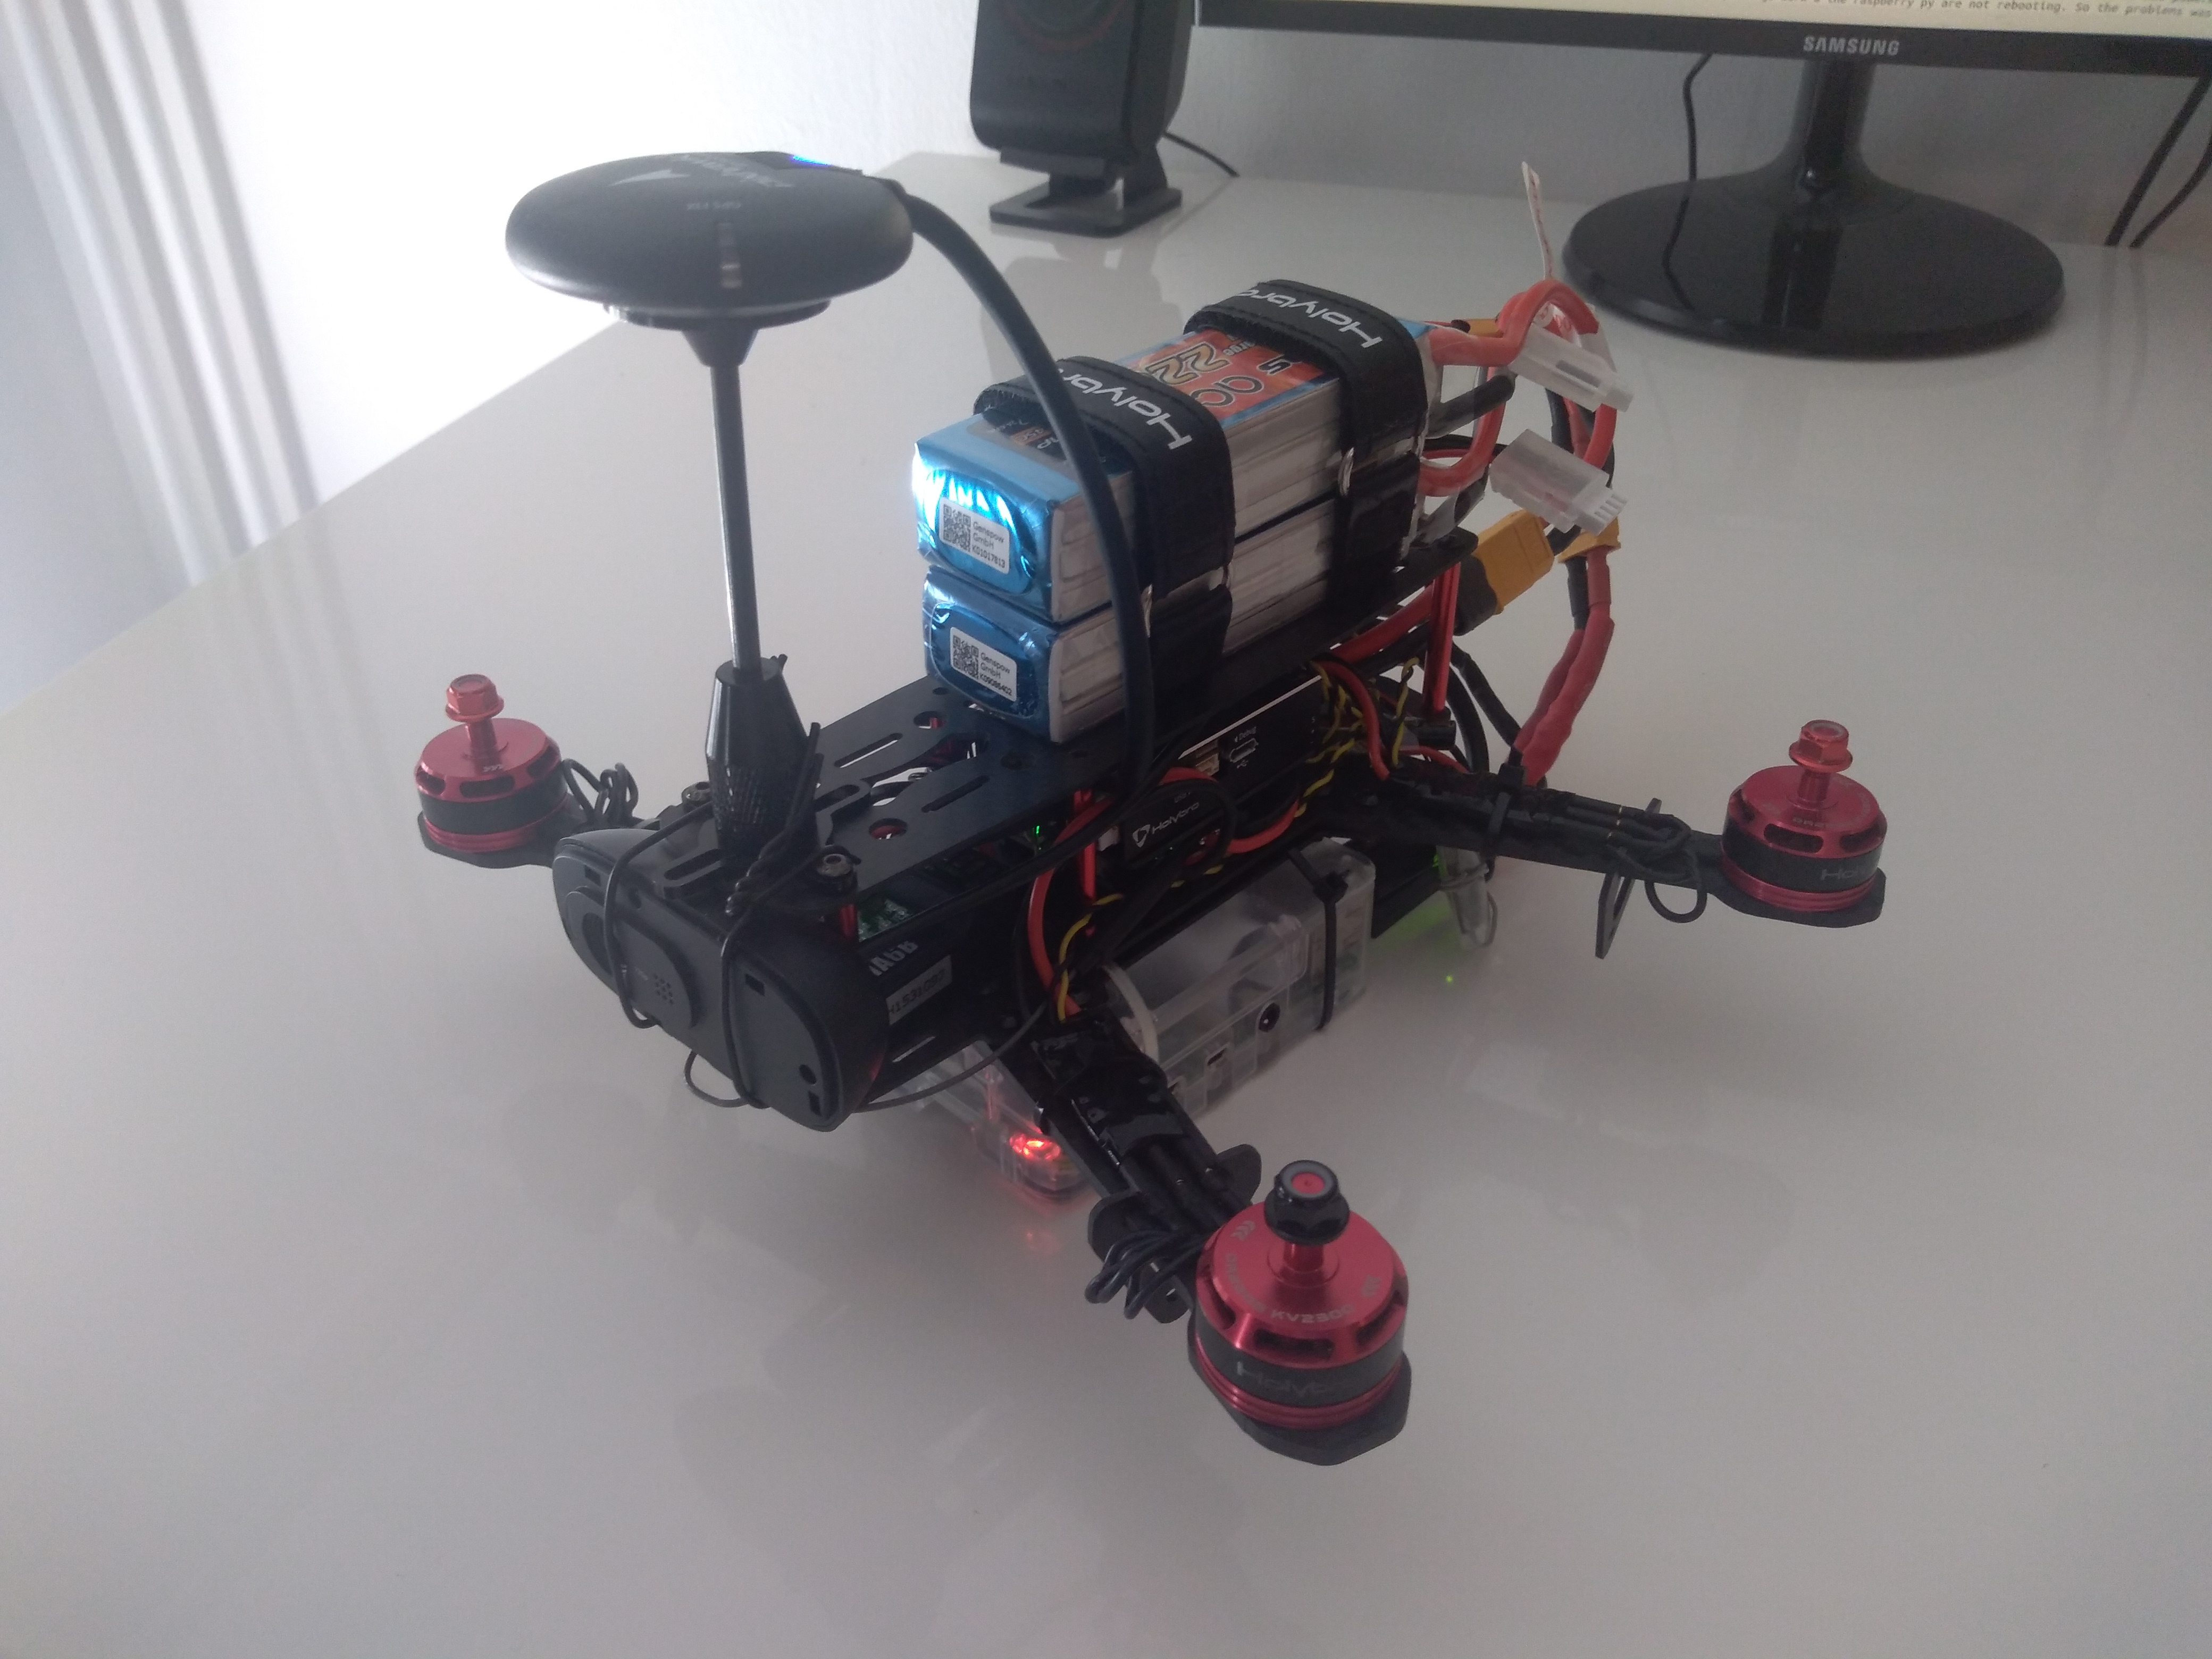
\includegraphics[height=3.5cm]{../Figures/without_landing_gear.jpg}
        \caption{}
        \label{fig:uav_without_landing_gear}
    \end{subfigure}
     \hspace{0.2em}
    \begin{subfigure}[t]{.30\textwidth}
        \centering
        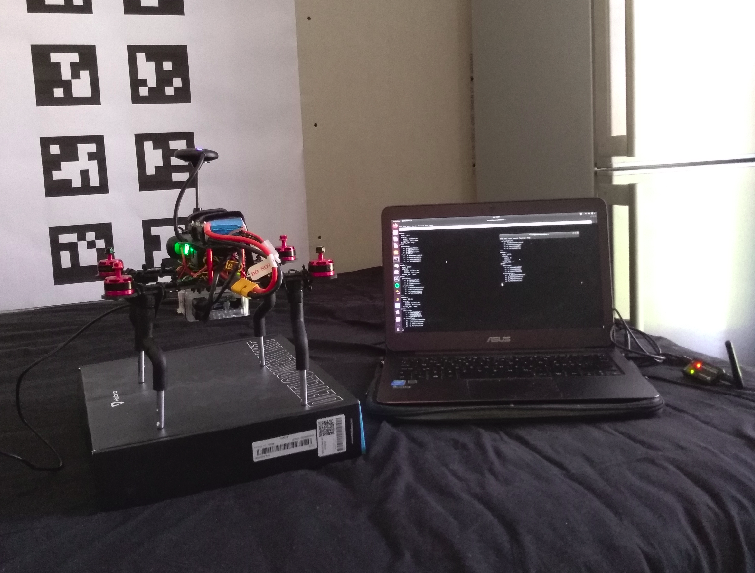
\includegraphics[height=3.5cm]{../Figures/initial_test_from_home.png}
        \caption{}
        \label{fig:uav_initial_test_from_home}
    \end{subfigure}
     \hspace{0.2em}
    \begin{subfigure}[t]{.30\textwidth}
        \centering
        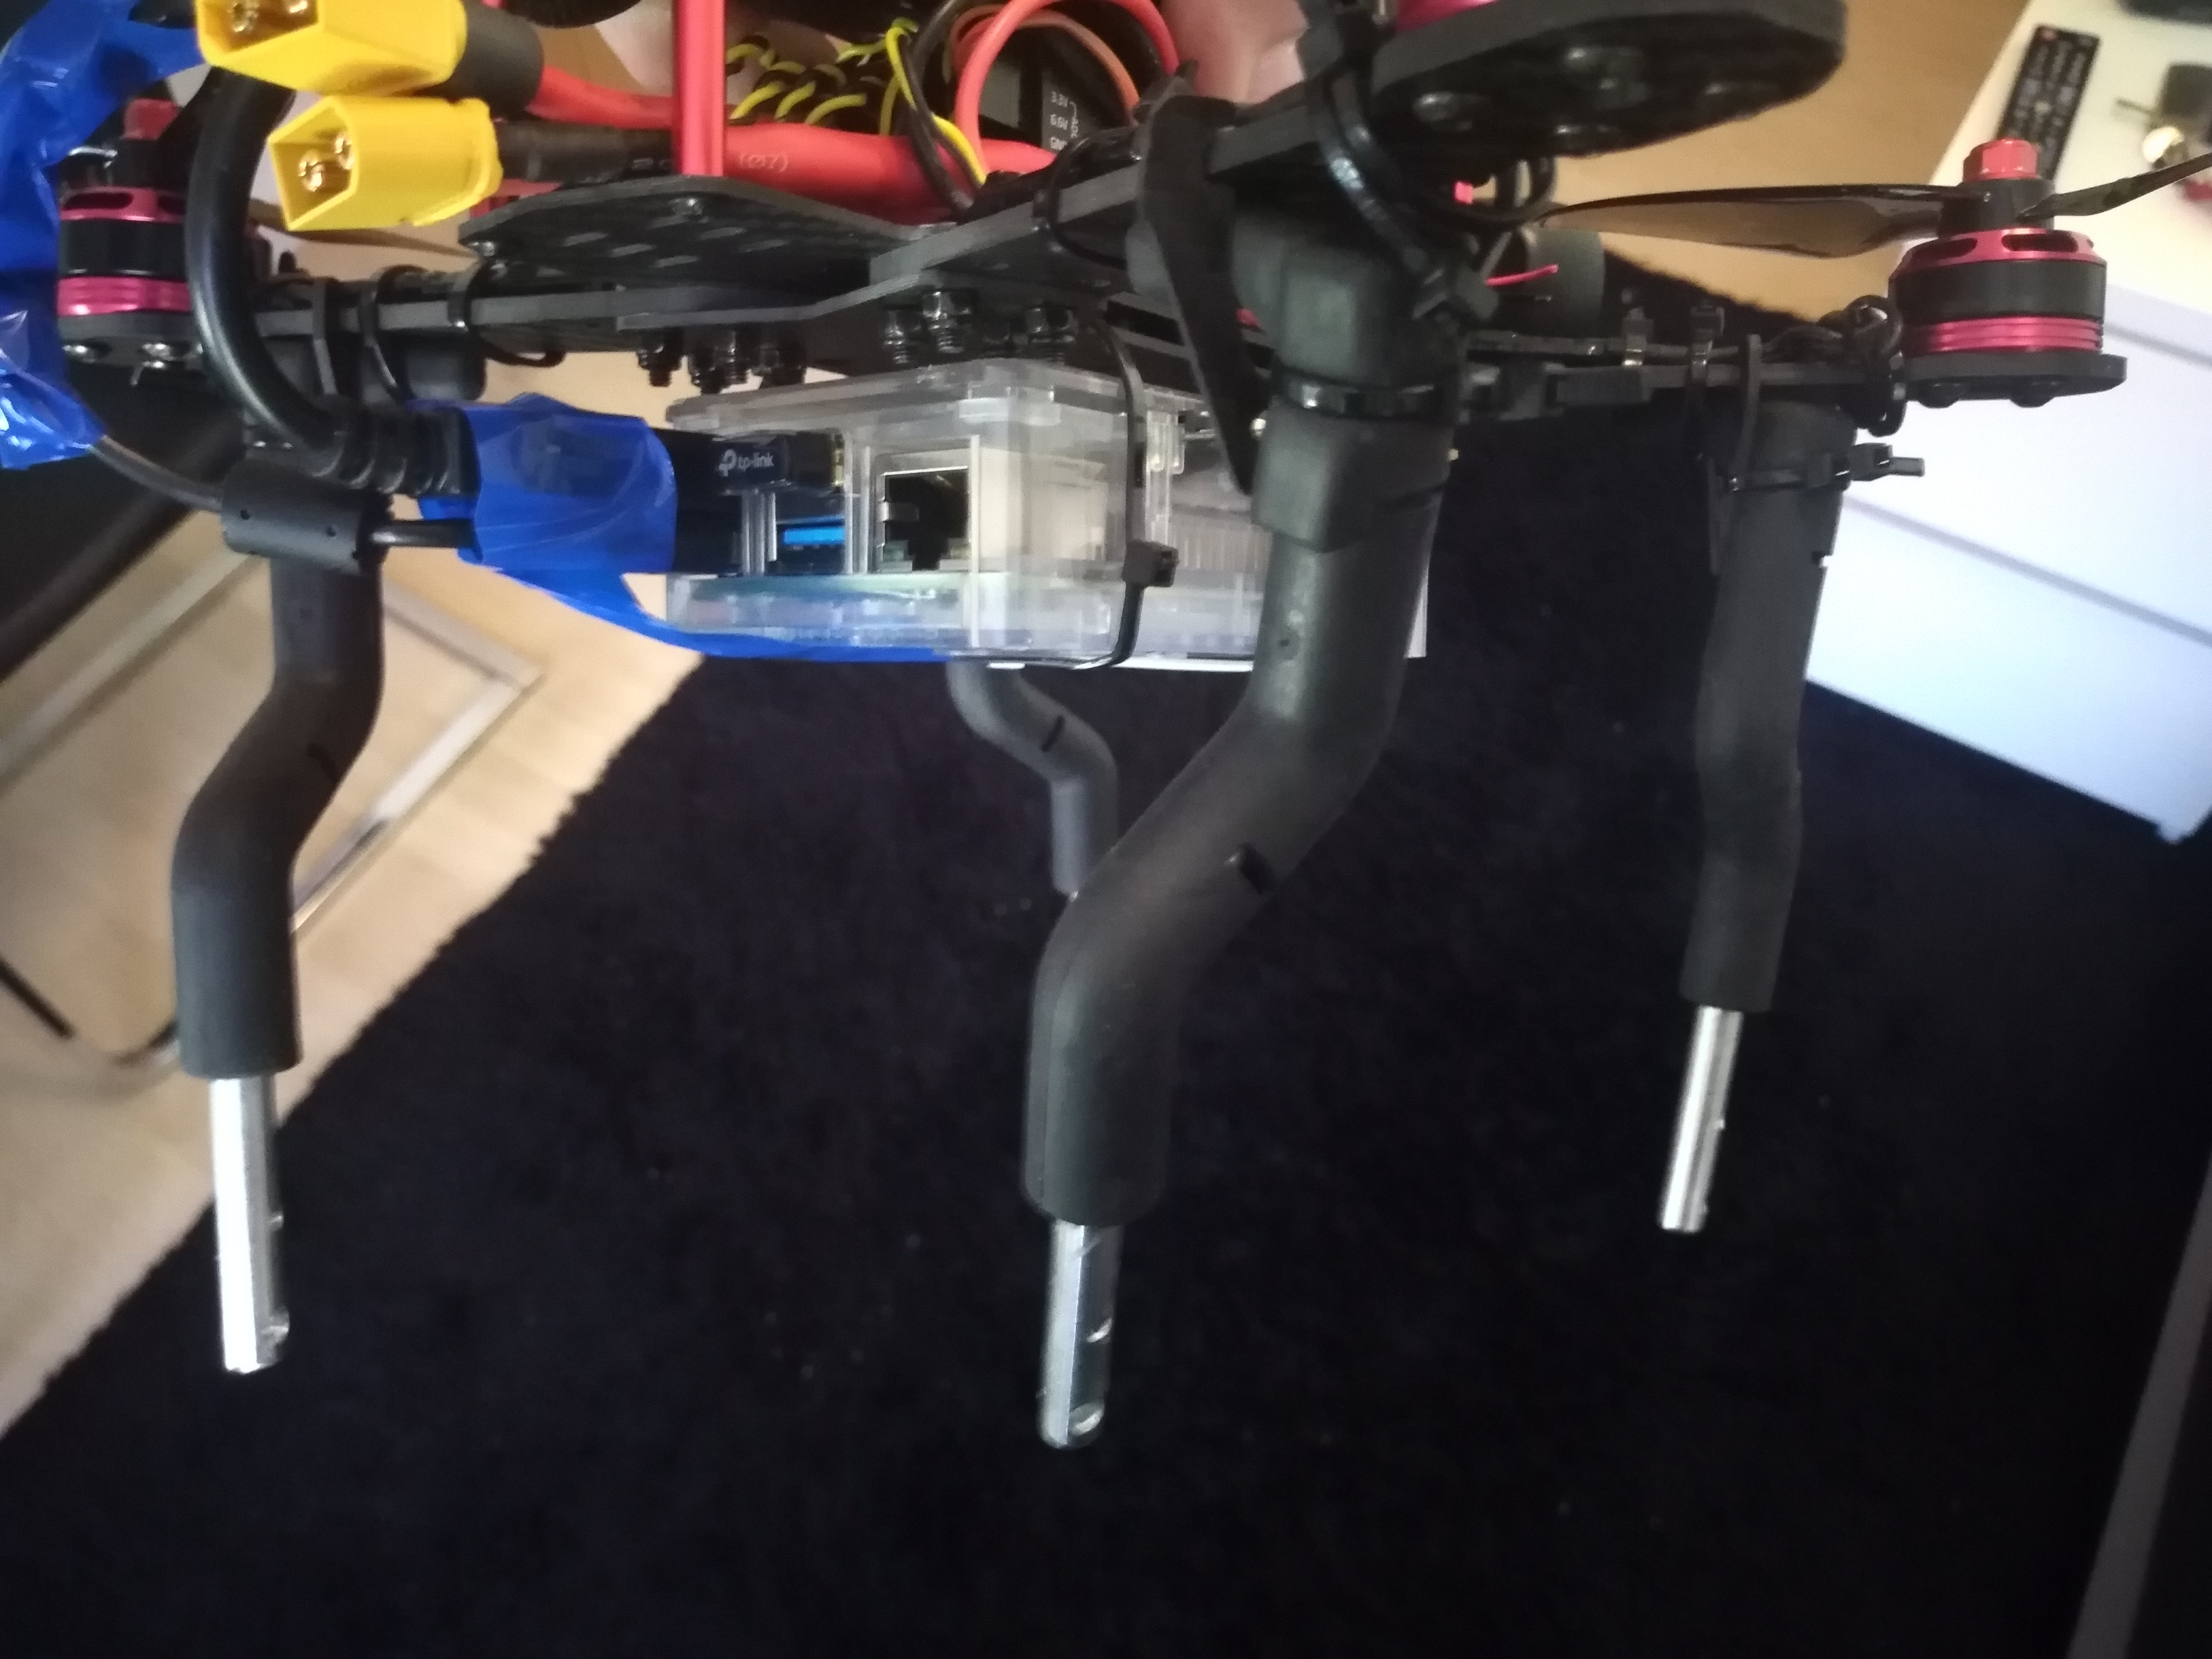
\includegraphics[height=3.5cm]{../Figures/damage_landing_gear.jpg}
        \caption{}
        \label{fig:uav_damage_landing_gear}
    \end{subfigure}
    \caption{Illustration of the UAV without the attached landing gear in Figure \ref{fig:uav_without_landing_gear}. Some of the initial testing of the vision based pose estimation and working with the UAV from home can be seen in Figure \ref{fig:uav_initial_test_from_home}. One of the legs can be seen to be bent after a number of vision based landings in the airport which can be seen in Figure \ref{fig:uav_damage_landing_gear}}
    \label{fig:general_challenges}
\end{figure}

However, without the landing gear there was no room for the Raspberry Pi as seen in Figure \ref{fig:uav_without_landing_gear}. Hence, this implementation was chosen thought not being optimal. As mentioned in Section \ref{sec:qgroundcontrol}, the use of the SDU drone would be the preferred solution, but due to time constrains, this was not implemented in the flight test in the OptiTrack system. Moreover, the UAV had a hard time flying with the two batteries attached as seen in Figure \ref{fig:uav_without_landing_gear}. This was because the center of mass being above the actual center of the UAV which led to instabilities. Hence, a wired power connection to the PX4 was attached to the UAV as seen in Figure \ref{fig:optitrack_hold_pose_boards} which solved the problem. Furthermore, it may the noticed that the UAV takes off quite slowly in the videos in Section \ref{sec:optitrack_hold_pose_using_estimated_aruco_pose} and \ref{sec:optitrack_vision_based_landing}. This is due to the extra load on the UAV e.g Raspberry Pi, landing gear etc. Improvements could be made by altering the default settings of the PID controllers in the PX4 autopilot. However, due to time constraints and the fact that the UAV was actually flying pretty well, though being slow, no change to the controllers was performed.  

\end{document}